\documentclass[10pt]{article}
% Standalone Supplementary Information with the main text's look. Folio
% builds it alongside main.tex. Each document reads the other's labels
% through xr: here main-text labels are M-..., in main.tex supplement labels
% are S-... (run both twice by hand for cross-document references to settle).

\usepackage[margin=1.9cm]{geometry}
\usepackage{graphicx}
\usepackage{booktabs}
\usepackage{array}
\usepackage{longtable}
\usepackage{amsmath}
% Same fonts as main.tex.
\usepackage{iftex}
\ifPDFTeX
  \usepackage[T1]{fontenc}
  \usepackage{helvet}
  \usepackage{courier}
  \DeclareUnicodeCharacter{2212}{\textminus}
  \DeclareUnicodeCharacter{2265}{\ensuremath{\geq}}
  \DeclareUnicodeCharacter{2264}{\ensuremath{\leq}}
  \DeclareUnicodeCharacter{2248}{\ensuremath{\approx}}
  \DeclareUnicodeCharacter{03B1}{\ensuremath{\alpha}}
  \DeclareUnicodeCharacter{2009}{\,}
\else
  \usepackage{fontspec}
  % By file name, so the fonts shipped with TeX Live are found on every system.
  \setsansfont{texgyreheros}[Extension=.otf, UprightFont=*-regular,
    BoldFont=*-bold, ItalicFont=*-italic, BoldItalicFont=*-bolditalic]
  \setmonofont{texgyrecursor}[Extension=.otf, UprightFont=*-regular,
    BoldFont=*-bold, ItalicFont=*-italic, BoldItalicFont=*-bolditalic]
\fi
\renewcommand{\familydefault}{\sfdefault}
\usepackage[italic]{mathastext}
\usepackage{rotating}
\usepackage{caption}

\usepackage{xr-hyper}
\usepackage[hidelinks]{hyperref}
\renewcommand{\UrlFont}{\ttfamily}
\usepackage{cleveref}
\externaldocument[M-]{main}
\usepackage[super,sort&compress]{natbib}
\usepackage{xcolor}
\usepackage{tikz}
\usetikzlibrary{positioning,calc,arrows.meta}
% Supplementary Notes: numbered, so they can be cited with \ref and \cref.
\newcounter{suppnote}
\crefname{figure}{Figure}{Figures}
\crefname{table}{Table}{Tables}
\crefname{suppnote}{Note}{Notes}
\newcommand{\tbd}[1]{\textcolor{red}{[#1]}}

\graphicspath{{figures/}}
\setcounter{secnumdepth}{0}

% Supplementary Figure S1, Table S1, ...
\renewcommand{\thefigure}{S\arabic{figure}}
\renewcommand{\thetable}{S\arabic{table}}

\begin{document}

\begin{center}
{\Large\bfseries Supplementary Information}\\[1ex]
{\large Title of the paper}\\[1ex]
First Author, Second Author
\end{center}

\begin{figure}[htbp]
\centering
% A TikZ figure kept as source; a script can regenerate it.
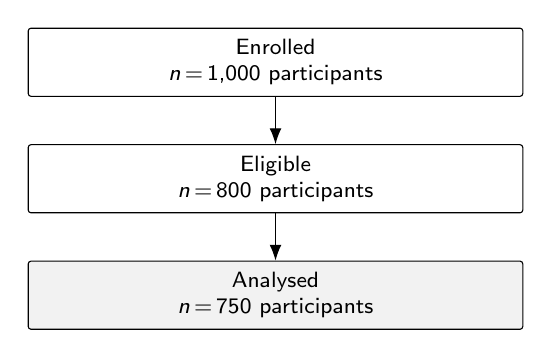
\begin{tikzpicture}[font=\footnotesize, node distance=6mm,
  box/.style={draw, rounded corners=1pt, align=center, text width=6cm, inner sep=4pt},
  arr/.style={-{Latex[length=2mm]}}]
\node[box] (all) {Enrolled\\\textit{n}\,=\,1,000 participants};
\node[box, below=of all] (elig) {Eligible\\\textit{n}\,=\,800 participants};
\node[box, below=of elig, fill=gray!10] (final) {Analysed\\\textit{n}\,=\,750 participants};
\draw[arr] (all) -- (elig);
\draw[arr] (elig) -- (final);
\end{tikzpicture}

\caption{Participant flow. A TikZ figure kept as source in
\texttt{figures/flow.tex}, so it can be regenerated by a script.}
\label{fig:supp-flow}
\end{figure}

\begin{table}[htbp]
\centering
\footnotesize
\caption{Model specifications. Each row is one analysis reported in the main
text.}
\label{tab:supp-details}
\begin{tabular}{@{}>{\raggedright\arraybackslash}p{3cm}>{\raggedright\arraybackslash}p{7cm}>{\raggedright\arraybackslash}p{4cm}@{}}
\toprule
\textbf{Analysis} & \textbf{Model} & \textbf{Reported in} \\
\midrule
Main finding & \texttt{y \textasciitilde{} method + (1 | subject)} & \cref{M-tab:results} \\ \addlinespace
Secondary finding & \texttt{y \textasciitilde{} method * group + (1 | subject)} & \cref{M-fig:overview}b \\
\bottomrule
\end{tabular}
\end{table}


\refstepcounter{suppnote}\label{note:supp-method}
\subsection*{Supplementary Note \thesuppnote: additional method}
Describe a method or analysis that does not fit the main text. It refers back
to the paper's \cref{M-tab:results} and \cref{M-fig:overview}, and to
\cref{tab:supp-details} in this document, and can cite~\cite{example2023book}.

\bibliographystyle{naturemag}
\bibliography{references}

\end{document}
